\documentclass[12pt]{article}
\usepackage[utf8]{inputenc}
\usepackage{graphicx}
\graphicspath{ {uml/rendered/} }

\begin{document}

Głównym elementem architektury są obiekty (agregaty), które reprezentują pewne elementy
świata gry w sposób, w jaki widzi je użytkownik.

\begin{figure}[h]
  \centering
  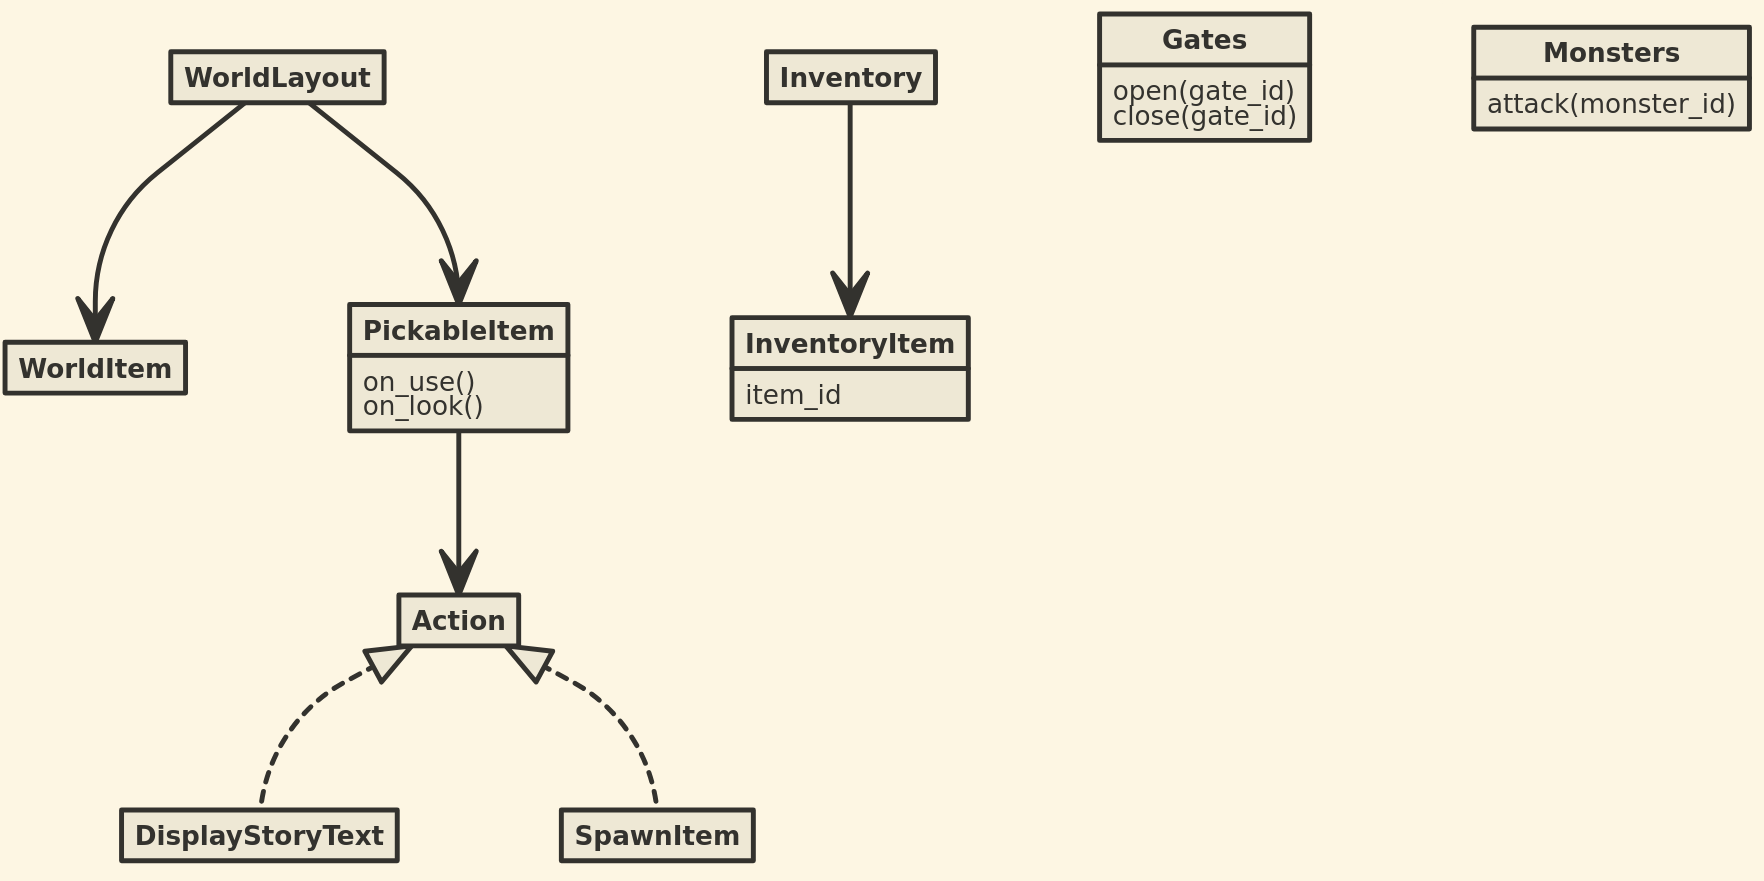
\includegraphics[width=\textwidth]{aggregates}
\end{figure}

Komunikują się między sobą poprzez przesyłanie powiadomień o:

\begin{itemize}
\item Poleceniach, reprezentujących intencję użytkownika lub obiektu, by coś zrobić
\item Zapytaniach, reprezentujących intencję użytkownika lub obiektu, by
  się czegoś dowiedzieć
\item Zdarzeniach, reprezentujących fakt, że coś się stało (np gracz podniósł
  przedmiot, drzwi zostały otwarte)
\end{itemize}

\begin{figure}[h]
  \centering
  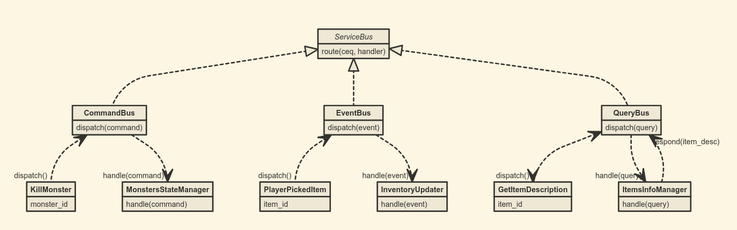
\includegraphics[width=\textwidth]{messaging}
\end{figure}

Właściwa gra jest definiowana w deklaratywny sposób, na przykład za pomocą YAML,
a stan gry daje się zapisać przy pomocy zewnetrznych źródeł, np zserializowanych obiektów.

\begin{figure}[h]
  \centering
  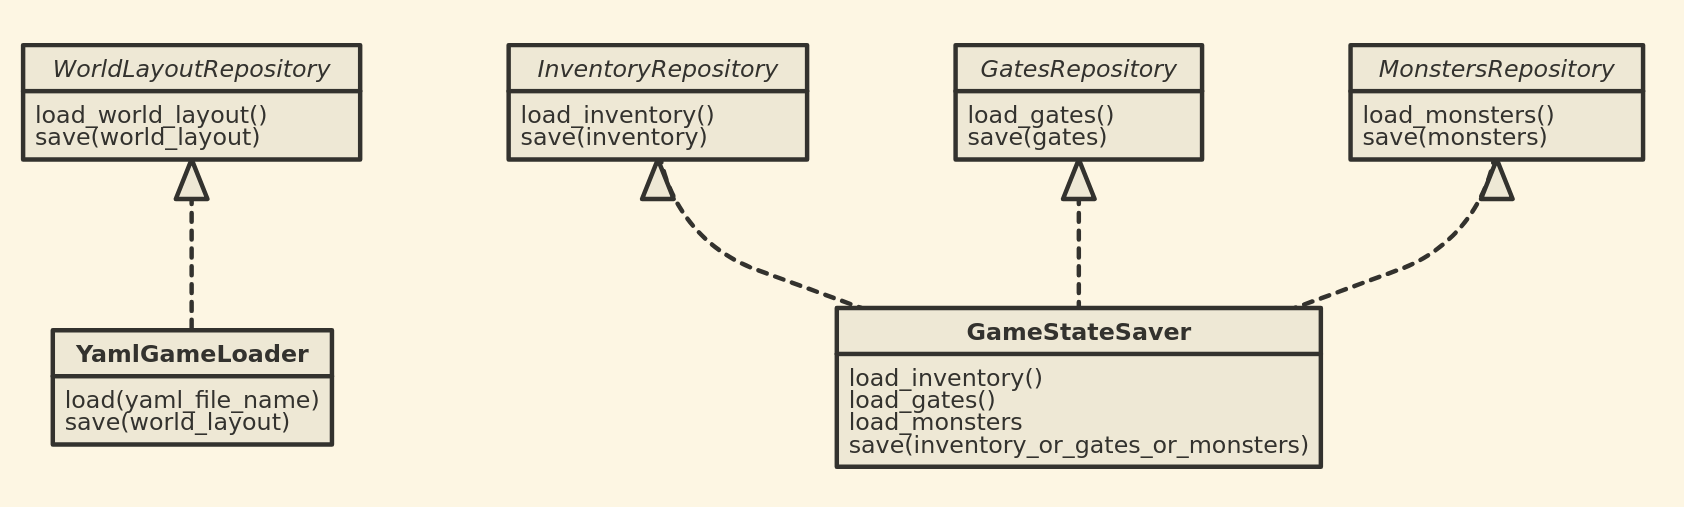
\includegraphics[width=\textwidth]{repositories}
\end{figure}

\end{document}